%%%%%%%%%%%%%%%%%%%%%%%%%%%%%%%%%%%%%%%%%%%%%%%%%%%%%%%%%%%%%%%%%%%%%%
%%                     Equivalence Arc
%%%%%%%%%%%%%%%%%%%%%%%%%%%%%%%%%%%%%%%%%%%%%%%%%%%%%%%%%%%%%%%%%%%%%%
%\color{blue}
\subsection{Glyph: \glyph{Equivalence arc} }\label{sec:equivalenceArc}

\glyph{Equivalence Arc} is the arc used to represent the fact that all entities
marked by a \glyph{tag} are equivalent. 

\begin{glyphDescription}
 \glyphSboTerm To be determined.
 \glyphOrigin Any \glyph{EPN} (\sect{EPNs}).
 \glyphTarget \glyph{Tag} (\sect{tag}).
 \glyphEndPoint No particular symbol is used to represent an \glyph{equivalence arc}.
 \end{glyphDescription}

\begin{figure}[H]
  \centering
  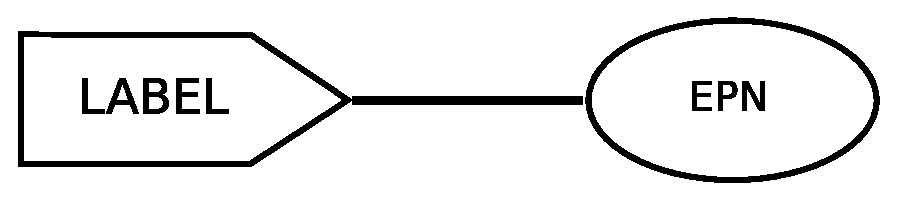
\includegraphics[scale = 0.4]{images/equivalence}
  \caption{The \PD glyph for \glyph{Equivalence arc}.}
  \label{fig:equivalence}
\end{figure}
